\documentclass{beamer}

\setbeamertemplate{bibliography item}{\insertbiblabel}
\usetheme{PaloAlto}
\makeatletter
\setlength{\beamer@headheight}{1cm}
\makeatother
\setbeamertemplate{navigation symbols}{}
\usepackage[absolute,overlay]{textpos}

\title[Advies WBH 02B09]{Hoe presteert de akoestiek van WBH 02B09?}
\subtitle{Een controle op de akoestieke normen}
\author{Alexander Arutunian (Team 4)}
\institute[HvA]{Hogeschool van Amsterdam}
\date{5 April, 2024}



\begin{document}

\begin{frame}
\titlepage
\end{frame}

% TABLE OF CONTENTS

\begin{frame}
\frametitle{Inhoudsopgaven}
\tableofcontents[pausesections]
\end{frame}


% INLEIDING
\section{Inleiding}

\subsection{Opdracht}

\begin{frame}{Inleiding}
\begin{block}{Opdracht}
Een collegezaal controleren op een van de akoestische eisen van een collegezaal, in ons geval de nagalmtijd.
\end{block}
\end{frame}

\subsection{Ruimte}

\begin{frame}{Inleiding}
\begin{block}{Opdracht}
Een collegezaal controleren op een van de akoestische eisen van een collegezaal, in ons geval de nagalmtijd.
\end{block}
\begin{block}{Ruimte}
Wij hebben ervoor gekozen om WBH 02B09 door te meten.
\end{block}
\end{frame}

\subsection{Adviesvraag}

\begin{frame}{Inleiding}
\begin{block}{Opdracht}
Een collegezaal controleren op een van de akoestische eisen van een collegezaal, in ons geval de nagalmtijd.
\end{block}
\begin{block}{Ruimte}
Wij hebben ervoor gekozen om WBH 02B09 door te meten.
\end{block}
\begin{block}{Adviesvraag}
Is er een behoefte voor akoestische herinrichting van de zaal?
\end{block}
\end{frame}

\subsection{Plattegrond}

\begin{frame}
\frametitle{Inleiding}
\begin{figure}
  \includegraphics[scale=0.6]{plattegrond}
  \caption{Plattegrond WBH 02B09$^{[1]}$}
\end{figure}
\end{frame}




% CONTEXTANALYSE
\section{Contextanalyse}
\subsection{Situatie en Complicaties}
\begin{frame}{Contextanalyse}
\begin{block}{Situatie en Complicaties}
  - Grote collegezaal.\\
  - Geen akoestische hulpmiddelen (bijv. diffusors).\\
  - Hele grote open ruimte op de plek waar de spreker staat.\\
  - Speaker systeem.\\
  - Stoelen die dun en minimalistisch zijn.
\end{block}
\end{frame}

\subsection{Functie van deze ruimte}
\begin{frame}{Contextanalyse}
\frametitle{Contextanalyse}
\begin{block}{Situatie en Complicaties}
  - Grote collegezaal.\\
  - Geen akoestische hulpmiddelen (bijv. diffusors).\\
  - Hele grote open ruimte op de plek waar de spreker staat.\\
  - Speaker systeem.\\
  - Stoelen die dun en minimalistisch zijn.
\end{block}
\begin{block}{Functie van deze ruimte}
  Uiteraard wordt dit gebruikt voor lessen, maar bijboorbeeld ook voor gastlezingen, uitreikingen en presentaties.
\end{block}
\end{frame}

\subsection{Verwachtingen van de opdrachtgever}
\begin{frame}{Contextanalyse}
\frametitle{Contextanalyse}
\begin{block}{Situatie en Complicaties}
  - Grote collegezaal.\\
  - Geen akoestische hulpmiddelen (bijv. diffusors).\\
  - Hele grote open ruimte op de plek waar de spreker staat.\\
  - Speaker systeem.\\
  - Stoelen die dun en minimalistisch zijn.
\end{block}
\begin{block}{Functie van deze ruimte}
  Uiteraard wordt dit gebruikt voor lessen, maar bijboorbeeld ook voor gastlezingen, uitreikingen en presentaties.
\end{block}
\begin{block}{Verwachtingen van de opdrachtgever}
  Een akoestiek die binnen de norm (0,7-0,9 sec)$^{[2]}$ valt. 
\end{block}
\end{frame}



% METHODE
\section{Methode}
\subsection{Hoe we hebben gemeten}
\begin{frame}
  \frametitle{Methode}
\begin{block}{Hoe we hebben gemeten}
  Elke stoel, 8 rijen, 17 stoelen per rij. Totaal 136 stoelen. Per stoel doen wij drie metingen, in totaal 408 metingen.
\end{block}
\begin{figure}
  \includegraphics[scale=0.1]{zaal}
\end{figure}
\end{frame}

\subsection{Verwijzingen}
\begin{frame}
  \frametitle{Methode}
\begin{block}{Hoe we hebben gemeten}
  Elke stoel, 8 rijen, 17 stoelen per rij. Totaal 136 stoelen. Per stoel doen wij drie metingen, in totaal 408 metingen.
\end{block}
\begin{figure}
  \includegraphics[scale=0.1]{zaal}
\end{figure}
\begin{block}{Verwijzingen}
  Voor meer detail zie meetplan en documentatie van meetinstrument.
\end{block}
\end{frame}

% RESULTATEN
\section{Resultaten}
\subsection{Betrouwbaarheid}
\begin{frame}{Resultaten}
\begin{block}{Betrouwbaarheid}
 - Personen in de zaal\\
 - Microfoon gebruik\\
 - Positie spreker\\
 - Kalibratierapport
\end{block}
\end{frame}
\begin{frame}{Resultaten}
\begin{textblock*}{5cm}(1.6cm,2cm)
  \begin{figure}
  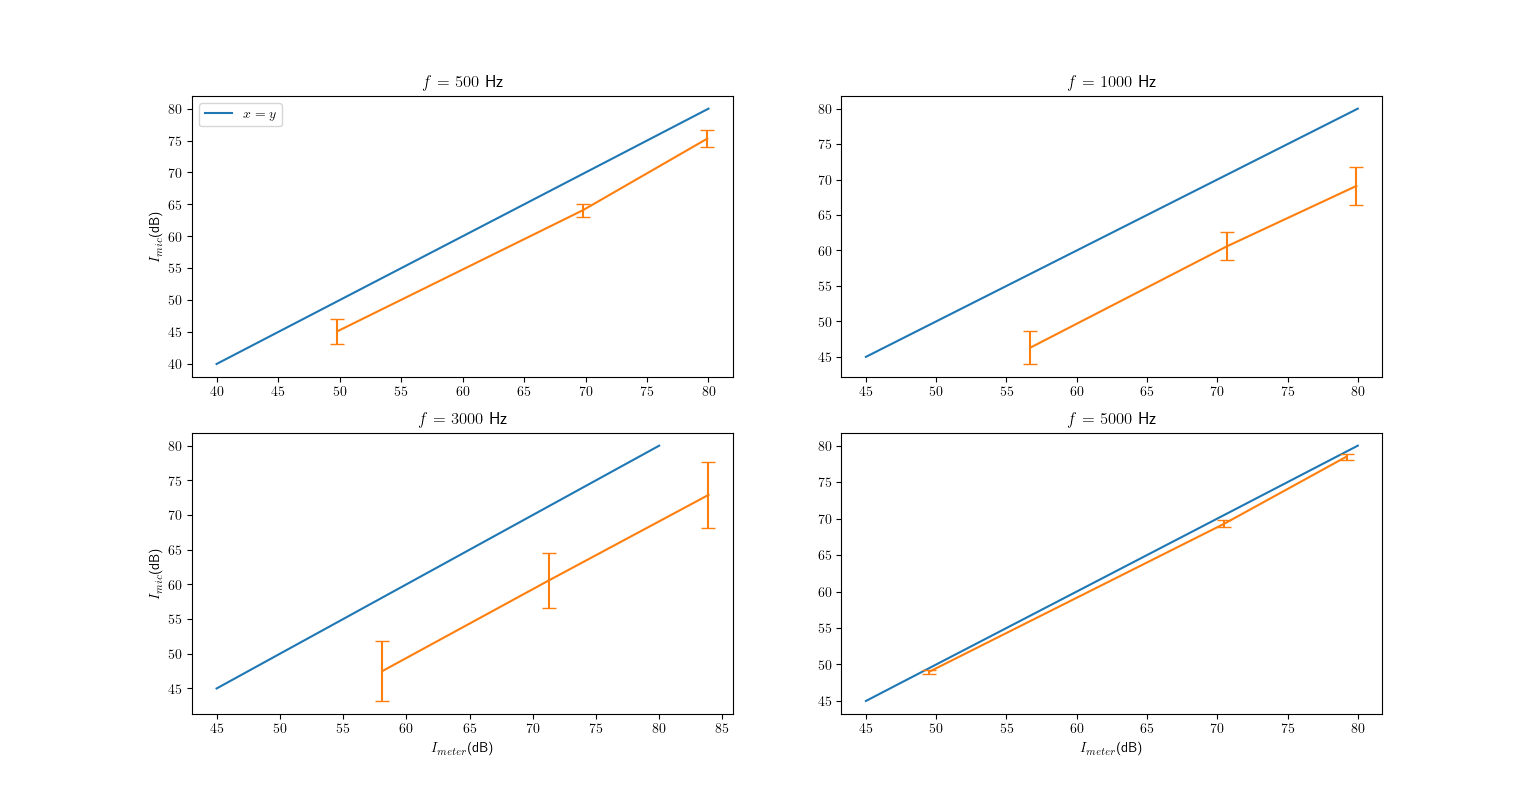
\includegraphics[scale=.35]{Figure_1}
  \caption{r1-s1-t3.wav, dB over tijd}
\end{figure}
\end{textblock*}
\end{frame}

\subsection{Heatmap}
\begin{frame}{Resultaten}
\begin{textblock*}{5cm}(1.7cm,1cm)
  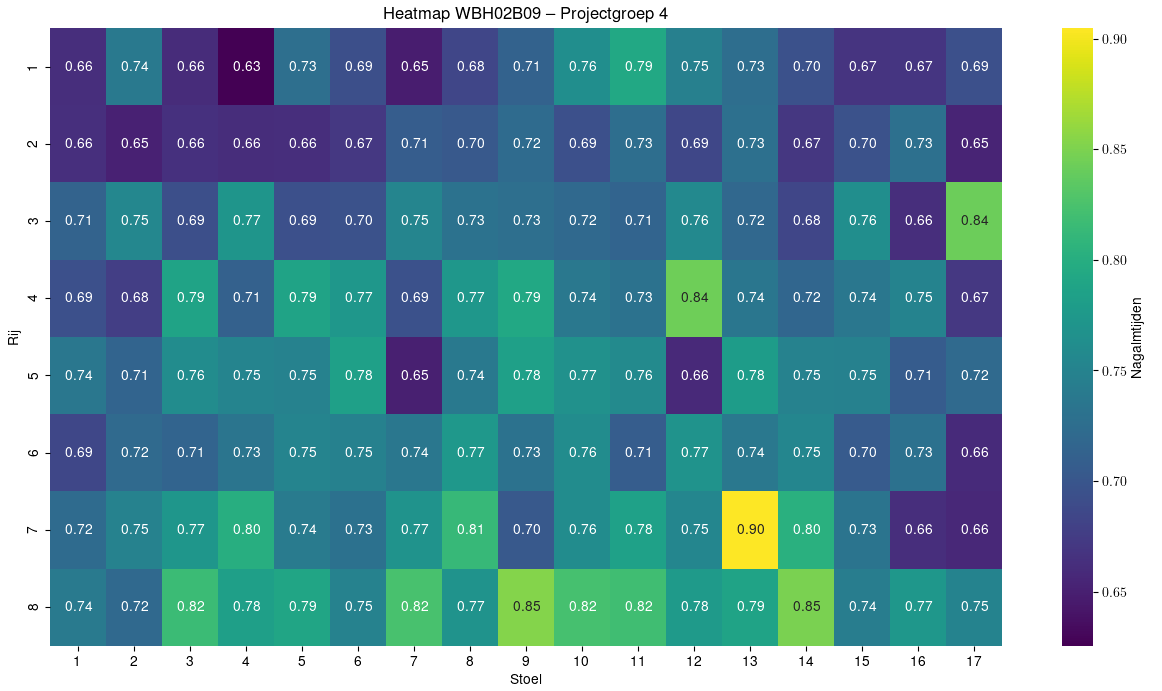
\includegraphics[scale=.37]{heatmap}
\end{textblock*}
\begin{textblock*}{8cm}(2cm,7.5cm)
\begin{block}{De norm voor collegezalen}
  0,7 tot 0,9 seconde$^{[2]}$
\end{block}
\end{textblock*}
\end{frame}


% ADVIES EN AANBEVELINGEN
\section{Advies en aanbevelingen}
\begin{frame}{Advies en aanbevelingen}
  \begin{block}{Gemiddelde nagalmtijd}
    De gemiddelde nagalmtijd van deze collegezaal is 0,7322 seconden.
  \end{block}
  \pause
  \begin{block}{Alternatieve metingen/Verdere onderzoek}
  - Simuleren hoe het zou zijn wanneer de zaal vol zou zitten, met bijvoorbeeld life-sized knuffels of grote kussens.\\
  - Meer ruimtes controleren op nagalmtijd.\\
  - Frequentie en intensiteiten gebruiken die overeenkomen met de stem van een mens.\\
  - Meten wanneer er gebruik wordt gemaakt van het speaker systeem.
 \end{block} 
\end{frame}




% BRONNEN
\section{Bronnen}
\begin{frame}[shrink=30]{Bronnen}
  \begin{thebibliography}{9}

    \bibitem{lamport94} 
 HVA WIBAUTHUIS, 2E ETAGE. https://www.hva.nl/binaries/content/assets/subsites/amstelcampus/plattegronden/wbh---2e-verd-ingevuld-kleuren.pdf?1429532947970
    \bibitem{lamport94}
    G. R. Ingenieurs, “Zaal- en ruimteakoestiek”. https://www.greten.nl/zaalenruimteakoestiek

\end{thebibliography}
\end{frame}

\end{document}






